% GNUPLOT: LaTeX picture with Postscript
\begingroup
  \makeatletter
  \providecommand\color[2][]{%
    \GenericError{(gnuplot) \space\space\space\@spaces}{%
      Package color not loaded in conjunction with
      terminal option `colourtext'%
    }{See the gnuplot documentation for explanation.%
    }{Either use 'blacktext' in gnuplot or load the package
      color.sty in LaTeX.}%
    \renewcommand\color[2][]{}%
  }%
  \providecommand\includegraphics[2][]{%
    \GenericError{(gnuplot) \space\space\space\@spaces}{%
      Package graphicx or graphics not loaded%
    }{See the gnuplot documentation for explanation.%
    }{The gnuplot epslatex terminal needs graphicx.sty or graphics.sty.}%
    \renewcommand\includegraphics[2][]{}%
  }%
  \providecommand\rotatebox[2]{#2}%
  \@ifundefined{ifGPcolor}{%
    \newif\ifGPcolor
    \GPcolortrue
  }{}%
  \@ifundefined{ifGPblacktext}{%
    \newif\ifGPblacktext
    \GPblacktexttrue
  }{}%
  % define a \g@addto@macro without @ in the name:
  \let\gplgaddtomacro\g@addto@macro
  % define empty templates for all commands taking text:
  \gdef\gplbacktext{}%
  \gdef\gplfronttext{}%
  \makeatother
  \ifGPblacktext
    % no textcolor at all
    \def\colorrgb#1{}%
    \def\colorgray#1{}%
  \else
    % gray or color?
    \ifGPcolor
      \def\colorrgb#1{\color[rgb]{#1}}%
      \def\colorgray#1{\color[gray]{#1}}%
      \expandafter\def\csname LTw\endcsname{\color{white}}%
      \expandafter\def\csname LTb\endcsname{\color{black}}%
      \expandafter\def\csname LTa\endcsname{\color{black}}%
      \expandafter\def\csname LT0\endcsname{\color[rgb]{1,0,0}}%
      \expandafter\def\csname LT1\endcsname{\color[rgb]{0,1,0}}%
      \expandafter\def\csname LT2\endcsname{\color[rgb]{0,0,1}}%
      \expandafter\def\csname LT3\endcsname{\color[rgb]{1,0,1}}%
      \expandafter\def\csname LT4\endcsname{\color[rgb]{0,1,1}}%
      \expandafter\def\csname LT5\endcsname{\color[rgb]{1,1,0}}%
      \expandafter\def\csname LT6\endcsname{\color[rgb]{0,0,0}}%
      \expandafter\def\csname LT7\endcsname{\color[rgb]{1,0.3,0}}%
      \expandafter\def\csname LT8\endcsname{\color[rgb]{0.5,0.5,0.5}}%
    \else
      % gray
      \def\colorrgb#1{\color{black}}%
      \def\colorgray#1{\color[gray]{#1}}%
      \expandafter\def\csname LTw\endcsname{\color{white}}%
      \expandafter\def\csname LTb\endcsname{\color{black}}%
      \expandafter\def\csname LTa\endcsname{\color{black}}%
      \expandafter\def\csname LT0\endcsname{\color{black}}%
      \expandafter\def\csname LT1\endcsname{\color{black}}%
      \expandafter\def\csname LT2\endcsname{\color{black}}%
      \expandafter\def\csname LT3\endcsname{\color{black}}%
      \expandafter\def\csname LT4\endcsname{\color{black}}%
      \expandafter\def\csname LT5\endcsname{\color{black}}%
      \expandafter\def\csname LT6\endcsname{\color{black}}%
      \expandafter\def\csname LT7\endcsname{\color{black}}%
      \expandafter\def\csname LT8\endcsname{\color{black}}%
    \fi
  \fi
    \setlength{\unitlength}{0.0500bp}%
    \ifx\gptboxheight\undefined%
      \newlength{\gptboxheight}%
      \newlength{\gptboxwidth}%
      \newsavebox{\gptboxtext}%
    \fi%
    \setlength{\fboxrule}{0.5pt}%
    \setlength{\fboxsep}{1pt}%
\begin{picture}(9620.00,9620.00)%
    \gplgaddtomacro\gplbacktext{%
      \csname LTb\endcsname%
      \put(840,6644){\makebox(0,0)[r]{\strut{}$10^{-3}$}}%
      \csname LTb\endcsname%
      \put(840,7036){\makebox(0,0)[r]{\strut{}$10^{-2}$}}%
      \csname LTb\endcsname%
      \put(840,7428){\makebox(0,0)[r]{\strut{}$10^{-1}$}}%
      \csname LTb\endcsname%
      \put(840,7820){\makebox(0,0)[r]{\strut{}$10^{0}$}}%
      \csname LTb\endcsname%
      \put(840,8212){\makebox(0,0)[r]{\strut{}$10^{1}$}}%
      \csname LTb\endcsname%
      \put(840,8604){\makebox(0,0)[r]{\strut{}$10^{2}$}}%
      \csname LTb\endcsname%
      \put(840,8996){\makebox(0,0)[r]{\strut{}$10^{3}$}}%
      \csname LTb\endcsname%
      \put(840,9388){\makebox(0,0)[r]{\strut{}$10^{4}$}}%
      \csname LTb\endcsname%
      \put(928,6445){\makebox(0,0){\strut{} }}%
      \csname LTb\endcsname%
      \put(1302,6445){\makebox(0,0){\strut{} }}%
      \csname LTb\endcsname%
      \put(1677,6445){\makebox(0,0){\strut{} }}%
      \csname LTb\endcsname%
      \put(2051,6445){\makebox(0,0){\strut{} }}%
      \csname LTb\endcsname%
      \put(2426,6445){\makebox(0,0){\strut{} }}%
      \csname LTb\endcsname%
      \put(2800,6445){\makebox(0,0){\strut{} }}%
      \csname LTb\endcsname%
      \put(3175,6445){\makebox(0,0){\strut{} }}%
      \csname LTb\endcsname%
      \put(3549,6445){\makebox(0,0){\strut{} }}%
      \csname LTb\endcsname%
      \put(3924,6445){\makebox(0,0){\strut{} }}%
      \csname LTb\endcsname%
      \put(4298,6445){\makebox(0,0){\strut{} }}%
      \csname LTb\endcsname%
      \put(4673,6445){\makebox(0,0){\strut{} }}%
      \csname LTb\endcsname%
      \put(4761,6644){\makebox(0,0)[l]{\strut{} }}%
      \csname LTb\endcsname%
      \put(4761,6918){\makebox(0,0)[l]{\strut{} }}%
      \csname LTb\endcsname%
      \put(4761,7193){\makebox(0,0)[l]{\strut{} }}%
      \csname LTb\endcsname%
      \put(4761,7467){\makebox(0,0)[l]{\strut{} }}%
      \csname LTb\endcsname%
      \put(4761,7742){\makebox(0,0)[l]{\strut{} }}%
      \csname LTb\endcsname%
      \put(4761,8016){\makebox(0,0)[l]{\strut{} }}%
      \csname LTb\endcsname%
      \put(4761,8290){\makebox(0,0)[l]{\strut{} }}%
      \csname LTb\endcsname%
      \put(4761,8565){\makebox(0,0)[l]{\strut{} }}%
      \csname LTb\endcsname%
      \put(4761,8839){\makebox(0,0)[l]{\strut{} }}%
      \csname LTb\endcsname%
      \put(4761,9114){\makebox(0,0)[l]{\strut{} }}%
      \csname LTb\endcsname%
      \put(4761,9388){\makebox(0,0)[l]{\strut{} }}%
      \csname LTb\endcsname%
      \put(928,9587){\makebox(0,0){\strut{}$10^{2}$}}%
      \csname LTb\endcsname%
      \put(1677,9587){\makebox(0,0){\strut{}$10^{3}$}}%
      \csname LTb\endcsname%
      \put(2426,9587){\makebox(0,0){\strut{}$10^{4}$}}%
      \csname LTb\endcsname%
      \put(3175,9587){\makebox(0,0){\strut{}$10^{5}$}}%
      \csname LTb\endcsname%
      \put(3924,9587){\makebox(0,0){\strut{}$10^{6}$}}%
      \csname LTb\endcsname%
      \put(4673,9587){\makebox(0,0){\strut{}$10^{7}$}}%
    }%
    \gplgaddtomacro\gplfronttext{%
      \csname LTb\endcsname%
      \put(300,8016){\rotatebox{-270}{\makebox(0,0){\strut{}$k = 2$}}}%
    }%
    \gplgaddtomacro\gplbacktext{%
      \csname LTb\endcsname%
      \put(4858,6644){\makebox(0,0)[r]{\strut{} }}%
      \csname LTb\endcsname%
      \put(4858,6918){\makebox(0,0)[r]{\strut{} }}%
      \csname LTb\endcsname%
      \put(4858,7193){\makebox(0,0)[r]{\strut{} }}%
      \csname LTb\endcsname%
      \put(4858,7467){\makebox(0,0)[r]{\strut{} }}%
      \csname LTb\endcsname%
      \put(4858,7742){\makebox(0,0)[r]{\strut{} }}%
      \csname LTb\endcsname%
      \put(4858,8016){\makebox(0,0)[r]{\strut{} }}%
      \csname LTb\endcsname%
      \put(4858,8290){\makebox(0,0)[r]{\strut{} }}%
      \csname LTb\endcsname%
      \put(4858,8565){\makebox(0,0)[r]{\strut{} }}%
      \csname LTb\endcsname%
      \put(4858,8839){\makebox(0,0)[r]{\strut{} }}%
      \csname LTb\endcsname%
      \put(4858,9114){\makebox(0,0)[r]{\strut{} }}%
      \csname LTb\endcsname%
      \put(4858,9388){\makebox(0,0)[r]{\strut{} }}%
      \csname LTb\endcsname%
      \put(4946,6445){\makebox(0,0){\strut{} }}%
      \csname LTb\endcsname%
      \put(5320,6445){\makebox(0,0){\strut{} }}%
      \csname LTb\endcsname%
      \put(5695,6445){\makebox(0,0){\strut{} }}%
      \csname LTb\endcsname%
      \put(6069,6445){\makebox(0,0){\strut{} }}%
      \csname LTb\endcsname%
      \put(6444,6445){\makebox(0,0){\strut{} }}%
      \csname LTb\endcsname%
      \put(6818,6445){\makebox(0,0){\strut{} }}%
      \csname LTb\endcsname%
      \put(7192,6445){\makebox(0,0){\strut{} }}%
      \csname LTb\endcsname%
      \put(7567,6445){\makebox(0,0){\strut{} }}%
      \csname LTb\endcsname%
      \put(7941,6445){\makebox(0,0){\strut{} }}%
      \csname LTb\endcsname%
      \put(8316,6445){\makebox(0,0){\strut{} }}%
      \csname LTb\endcsname%
      \put(8690,6445){\makebox(0,0){\strut{} }}%
      \csname LTb\endcsname%
      \put(8778,6644){\makebox(0,0)[l]{\strut{}$10^{-3}$}}%
      \csname LTb\endcsname%
      \put(8778,7036){\makebox(0,0)[l]{\strut{}$10^{-2}$}}%
      \csname LTb\endcsname%
      \put(8778,7428){\makebox(0,0)[l]{\strut{}$10^{-1}$}}%
      \csname LTb\endcsname%
      \put(8778,7820){\makebox(0,0)[l]{\strut{}$10^{0}$}}%
      \csname LTb\endcsname%
      \put(8778,8212){\makebox(0,0)[l]{\strut{}$10^{1}$}}%
      \csname LTb\endcsname%
      \put(8778,8604){\makebox(0,0)[l]{\strut{}$10^{2}$}}%
      \csname LTb\endcsname%
      \put(8778,8996){\makebox(0,0)[l]{\strut{}$10^{3}$}}%
      \csname LTb\endcsname%
      \put(8778,9388){\makebox(0,0)[l]{\strut{}$10^{4}$}}%
      \csname LTb\endcsname%
      \put(4946,9587){\makebox(0,0){\strut{}$10^{2}$}}%
      \csname LTb\endcsname%
      \put(5695,9587){\makebox(0,0){\strut{}$10^{3}$}}%
      \csname LTb\endcsname%
      \put(6444,9587){\makebox(0,0){\strut{}$10^{4}$}}%
      \csname LTb\endcsname%
      \put(7192,9587){\makebox(0,0){\strut{}$10^{5}$}}%
      \csname LTb\endcsname%
      \put(7941,9587){\makebox(0,0){\strut{}$10^{6}$}}%
      \csname LTb\endcsname%
      \put(8690,9587){\makebox(0,0){\strut{}$10^{7}$}}%
    }%
    \gplgaddtomacro\gplfronttext{%
      \csname LTb\endcsname%
      \put(9316,8016){\rotatebox{-270}{\makebox(0,0){\strut{}$k = 3$}}}%
    }%
    \gplgaddtomacro\gplbacktext{%
      \csname LTb\endcsname%
      \put(840,3437){\makebox(0,0)[r]{\strut{}$10^{-3}$}}%
      \csname LTb\endcsname%
      \put(840,3829){\makebox(0,0)[r]{\strut{}$10^{-2}$}}%
      \csname LTb\endcsname%
      \put(840,4221){\makebox(0,0)[r]{\strut{}$10^{-1}$}}%
      \csname LTb\endcsname%
      \put(840,4613){\makebox(0,0)[r]{\strut{}$10^{0}$}}%
      \csname LTb\endcsname%
      \put(840,5006){\makebox(0,0)[r]{\strut{}$10^{1}$}}%
      \csname LTb\endcsname%
      \put(840,5398){\makebox(0,0)[r]{\strut{}$10^{2}$}}%
      \csname LTb\endcsname%
      \put(840,5790){\makebox(0,0)[r]{\strut{}$10^{3}$}}%
      \csname LTb\endcsname%
      \put(840,6182){\makebox(0,0)[r]{\strut{}$10^{4}$}}%
      \csname LTb\endcsname%
      \put(928,3238){\makebox(0,0){\strut{} }}%
      \csname LTb\endcsname%
      \put(1677,3238){\makebox(0,0){\strut{} }}%
      \csname LTb\endcsname%
      \put(2426,3238){\makebox(0,0){\strut{} }}%
      \csname LTb\endcsname%
      \put(3175,3238){\makebox(0,0){\strut{} }}%
      \csname LTb\endcsname%
      \put(3924,3238){\makebox(0,0){\strut{} }}%
      \csname LTb\endcsname%
      \put(4673,3238){\makebox(0,0){\strut{} }}%
      \csname LTb\endcsname%
      \put(4761,3437){\makebox(0,0)[l]{\strut{} }}%
      \csname LTb\endcsname%
      \put(4761,3711){\makebox(0,0)[l]{\strut{} }}%
      \csname LTb\endcsname%
      \put(4761,3986){\makebox(0,0)[l]{\strut{} }}%
      \csname LTb\endcsname%
      \put(4761,4260){\makebox(0,0)[l]{\strut{} }}%
      \csname LTb\endcsname%
      \put(4761,4535){\makebox(0,0)[l]{\strut{} }}%
      \csname LTb\endcsname%
      \put(4761,4809){\makebox(0,0)[l]{\strut{} }}%
      \csname LTb\endcsname%
      \put(4761,5084){\makebox(0,0)[l]{\strut{} }}%
      \csname LTb\endcsname%
      \put(4761,5358){\makebox(0,0)[l]{\strut{} }}%
      \csname LTb\endcsname%
      \put(4761,5633){\makebox(0,0)[l]{\strut{} }}%
      \csname LTb\endcsname%
      \put(4761,5907){\makebox(0,0)[l]{\strut{} }}%
      \csname LTb\endcsname%
      \put(4761,6182){\makebox(0,0)[l]{\strut{} }}%
      \csname LTb\endcsname%
      \put(928,6381){\makebox(0,0){\strut{} }}%
      \csname LTb\endcsname%
      \put(1302,6381){\makebox(0,0){\strut{} }}%
      \csname LTb\endcsname%
      \put(1677,6381){\makebox(0,0){\strut{} }}%
      \csname LTb\endcsname%
      \put(2051,6381){\makebox(0,0){\strut{} }}%
      \csname LTb\endcsname%
      \put(2426,6381){\makebox(0,0){\strut{} }}%
      \csname LTb\endcsname%
      \put(2800,6381){\makebox(0,0){\strut{} }}%
      \csname LTb\endcsname%
      \put(3175,6381){\makebox(0,0){\strut{} }}%
      \csname LTb\endcsname%
      \put(3549,6381){\makebox(0,0){\strut{} }}%
      \csname LTb\endcsname%
      \put(3924,6381){\makebox(0,0){\strut{} }}%
      \csname LTb\endcsname%
      \put(4298,6381){\makebox(0,0){\strut{} }}%
      \csname LTb\endcsname%
      \put(4673,6381){\makebox(0,0){\strut{} }}%
    }%
    \gplgaddtomacro\gplfronttext{%
      \csname LTb\endcsname%
      \put(300,4809){\rotatebox{-270}{\makebox(0,0){\strut{}$k = 4$}}}%
    }%
    \gplgaddtomacro\gplbacktext{%
      \csname LTb\endcsname%
      \put(4858,3437){\makebox(0,0)[r]{\strut{} }}%
      \csname LTb\endcsname%
      \put(4858,3711){\makebox(0,0)[r]{\strut{} }}%
      \csname LTb\endcsname%
      \put(4858,3986){\makebox(0,0)[r]{\strut{} }}%
      \csname LTb\endcsname%
      \put(4858,4260){\makebox(0,0)[r]{\strut{} }}%
      \csname LTb\endcsname%
      \put(4858,4535){\makebox(0,0)[r]{\strut{} }}%
      \csname LTb\endcsname%
      \put(4858,4809){\makebox(0,0)[r]{\strut{} }}%
      \csname LTb\endcsname%
      \put(4858,5084){\makebox(0,0)[r]{\strut{} }}%
      \csname LTb\endcsname%
      \put(4858,5358){\makebox(0,0)[r]{\strut{} }}%
      \csname LTb\endcsname%
      \put(4858,5633){\makebox(0,0)[r]{\strut{} }}%
      \csname LTb\endcsname%
      \put(4858,5907){\makebox(0,0)[r]{\strut{} }}%
      \csname LTb\endcsname%
      \put(4858,6182){\makebox(0,0)[r]{\strut{} }}%
      \csname LTb\endcsname%
      \put(4946,3238){\makebox(0,0){\strut{}$10^{2}$}}%
      \csname LTb\endcsname%
      \put(5695,3238){\makebox(0,0){\strut{}$10^{3}$}}%
      \csname LTb\endcsname%
      \put(6444,3238){\makebox(0,0){\strut{}$10^{4}$}}%
      \csname LTb\endcsname%
      \put(7192,3238){\makebox(0,0){\strut{}$10^{5}$}}%
      \csname LTb\endcsname%
      \put(7941,3238){\makebox(0,0){\strut{}$10^{6}$}}%
      \csname LTb\endcsname%
      \put(8690,3238){\makebox(0,0){\strut{}$10^{7}$}}%
      \csname LTb\endcsname%
      \put(8778,3437){\makebox(0,0)[l]{\strut{}$10^{-3}$}}%
      \csname LTb\endcsname%
      \put(8778,3829){\makebox(0,0)[l]{\strut{}$10^{-2}$}}%
      \csname LTb\endcsname%
      \put(8778,4221){\makebox(0,0)[l]{\strut{}$10^{-1}$}}%
      \csname LTb\endcsname%
      \put(8778,4613){\makebox(0,0)[l]{\strut{}$10^{0}$}}%
      \csname LTb\endcsname%
      \put(8778,5006){\makebox(0,0)[l]{\strut{}$10^{1}$}}%
      \csname LTb\endcsname%
      \put(8778,5398){\makebox(0,0)[l]{\strut{}$10^{2}$}}%
      \csname LTb\endcsname%
      \put(8778,5790){\makebox(0,0)[l]{\strut{}$10^{3}$}}%
      \csname LTb\endcsname%
      \put(8778,6182){\makebox(0,0)[l]{\strut{}$10^{4}$}}%
      \csname LTb\endcsname%
      \put(4946,6381){\makebox(0,0){\strut{} }}%
      \csname LTb\endcsname%
      \put(5320,6381){\makebox(0,0){\strut{} }}%
      \csname LTb\endcsname%
      \put(5695,6381){\makebox(0,0){\strut{} }}%
      \csname LTb\endcsname%
      \put(6069,6381){\makebox(0,0){\strut{} }}%
      \csname LTb\endcsname%
      \put(6444,6381){\makebox(0,0){\strut{} }}%
      \csname LTb\endcsname%
      \put(6818,6381){\makebox(0,0){\strut{} }}%
      \csname LTb\endcsname%
      \put(7192,6381){\makebox(0,0){\strut{} }}%
      \csname LTb\endcsname%
      \put(7567,6381){\makebox(0,0){\strut{} }}%
      \csname LTb\endcsname%
      \put(7941,6381){\makebox(0,0){\strut{} }}%
      \csname LTb\endcsname%
      \put(8316,6381){\makebox(0,0){\strut{} }}%
      \csname LTb\endcsname%
      \put(8690,6381){\makebox(0,0){\strut{} }}%
    }%
    \gplgaddtomacro\gplfronttext{%
      \csname LTb\endcsname%
      \put(9316,4809){\rotatebox{-270}{\makebox(0,0){\strut{}$k = 5$}}}%
    }%
    \gplgaddtomacro\gplbacktext{%
      \csname LTb\endcsname%
      \put(840,231){\makebox(0,0)[r]{\strut{}$10^{-3}$}}%
      \csname LTb\endcsname%
      \put(840,623){\makebox(0,0)[r]{\strut{}$10^{-2}$}}%
      \csname LTb\endcsname%
      \put(840,1015){\makebox(0,0)[r]{\strut{}$10^{-1}$}}%
      \csname LTb\endcsname%
      \put(840,1407){\makebox(0,0)[r]{\strut{}$10^{0}$}}%
      \csname LTb\endcsname%
      \put(840,1799){\makebox(0,0)[r]{\strut{}$10^{1}$}}%
      \csname LTb\endcsname%
      \put(840,2191){\makebox(0,0)[r]{\strut{}$10^{2}$}}%
      \csname LTb\endcsname%
      \put(840,2583){\makebox(0,0)[r]{\strut{}$10^{3}$}}%
      \csname LTb\endcsname%
      \put(840,2975){\makebox(0,0)[r]{\strut{}$10^{4}$}}%
      \csname LTb\endcsname%
      \put(928,32){\makebox(0,0){\strut{}$10^{2}$}}%
      \csname LTb\endcsname%
      \put(1677,32){\makebox(0,0){\strut{}$10^{3}$}}%
      \csname LTb\endcsname%
      \put(2426,32){\makebox(0,0){\strut{}$10^{4}$}}%
      \csname LTb\endcsname%
      \put(3175,32){\makebox(0,0){\strut{}$10^{5}$}}%
      \csname LTb\endcsname%
      \put(3924,32){\makebox(0,0){\strut{}$10^{6}$}}%
      \csname LTb\endcsname%
      \put(4673,32){\makebox(0,0){\strut{}$10^{7}$}}%
      \csname LTb\endcsname%
      \put(4761,231){\makebox(0,0)[l]{\strut{} }}%
      \csname LTb\endcsname%
      \put(4761,505){\makebox(0,0)[l]{\strut{} }}%
      \csname LTb\endcsname%
      \put(4761,780){\makebox(0,0)[l]{\strut{} }}%
      \csname LTb\endcsname%
      \put(4761,1054){\makebox(0,0)[l]{\strut{} }}%
      \csname LTb\endcsname%
      \put(4761,1329){\makebox(0,0)[l]{\strut{} }}%
      \csname LTb\endcsname%
      \put(4761,1603){\makebox(0,0)[l]{\strut{} }}%
      \csname LTb\endcsname%
      \put(4761,1877){\makebox(0,0)[l]{\strut{} }}%
      \csname LTb\endcsname%
      \put(4761,2152){\makebox(0,0)[l]{\strut{} }}%
      \csname LTb\endcsname%
      \put(4761,2426){\makebox(0,0)[l]{\strut{} }}%
      \csname LTb\endcsname%
      \put(4761,2701){\makebox(0,0)[l]{\strut{} }}%
      \csname LTb\endcsname%
      \put(4761,2975){\makebox(0,0)[l]{\strut{} }}%
      \csname LTb\endcsname%
      \put(928,3174){\makebox(0,0){\strut{} }}%
      \csname LTb\endcsname%
      \put(1302,3174){\makebox(0,0){\strut{} }}%
      \csname LTb\endcsname%
      \put(1677,3174){\makebox(0,0){\strut{} }}%
      \csname LTb\endcsname%
      \put(2051,3174){\makebox(0,0){\strut{} }}%
      \csname LTb\endcsname%
      \put(2426,3174){\makebox(0,0){\strut{} }}%
      \csname LTb\endcsname%
      \put(2800,3174){\makebox(0,0){\strut{} }}%
      \csname LTb\endcsname%
      \put(3175,3174){\makebox(0,0){\strut{} }}%
      \csname LTb\endcsname%
      \put(3549,3174){\makebox(0,0){\strut{} }}%
      \csname LTb\endcsname%
      \put(3924,3174){\makebox(0,0){\strut{} }}%
      \csname LTb\endcsname%
      \put(4298,3174){\makebox(0,0){\strut{} }}%
      \csname LTb\endcsname%
      \put(4673,3174){\makebox(0,0){\strut{} }}%
    }%
    \gplgaddtomacro\gplfronttext{%
      \csname LTb\endcsname%
      \put(300,1603){\rotatebox{-270}{\makebox(0,0){\strut{}$k = 6$}}}%
      \csname LTb\endcsname%
      \put(7811,2875){\makebox(0,0)[r]{\strut{}Pardiso}}%
      \csname LTb\endcsname%
      \put(7811,2676){\makebox(0,0)[r]{\strut{}Mumps}}%
      \csname LTb\endcsname%
      \put(7811,2477){\makebox(0,0)[r]{\strut{}linear}}%
      \csname LTb\endcsname%
      \put(7811,2278){\makebox(0,0)[r]{\strut{}Mult Gr w Blk Jac}}%
      \csname LTb\endcsname%
      \put(7811,2079){\makebox(0,0)[r]{\strut{}Add Swz w Coarse}}%
      \csname LTb\endcsname%
      \put(7811,1880){\makebox(0,0)[r]{\strut{}Add Swz}}%
      \csname LTb\endcsname%
      \put(7811,1681){\makebox(0,0)[r]{\strut{}Pardiso w Blk PC}}%
      \csname LTb\endcsname%
      \put(7811,1482){\makebox(0,0)[r]{\strut{}CG}}%
    }%
    \gplbacktext
    \put(0,0){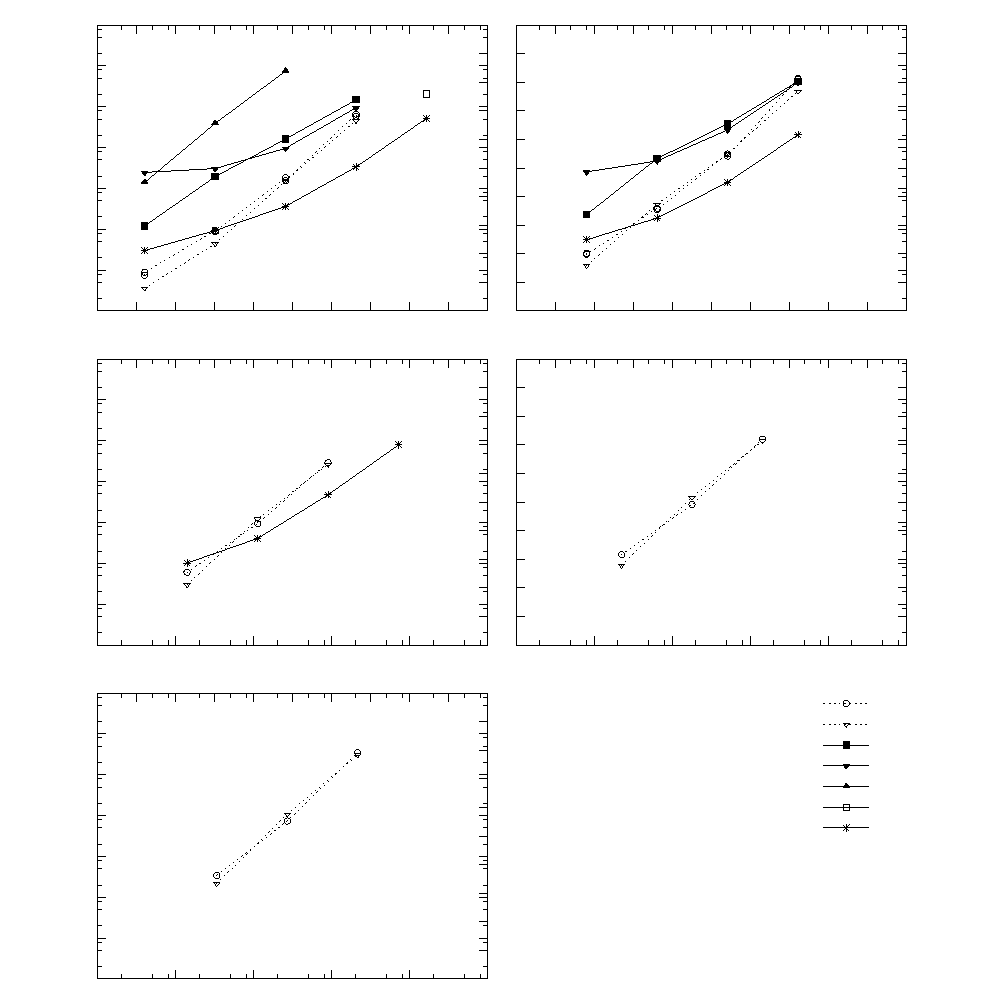
\includegraphics{ConstCoeffPoissonScaling}}%
    \gplfronttext
  \end{picture}%
\endgroup
